\documentclass[11pt,letterpaper]{article}
%\documentclass[11pt,letterpaper]{exam}
\usepackage[latin1]{inputenc}
\usepackage[left=3.00cm, right=3.00cm, top=3.00cm, bottom=3.00cm]{geometry}

\usepackage{amsmath}
%\usepackage{amsthm}
%\usepackage{cancel}
\usepackage{mathtools}
%\DeclarePairedDelimiter\ceil{\lceil}{\rceil}
%\DeclarePairedDelimiter\floor{\lfloor}{\rfloor}

\usepackage{fancyhdr}
\pagestyle{fancy}

\usepackage{color}
%\usepackage{xcolor}
\usepackage{graphicx}
\usepackage{caption}
%\definecolor{acolour}{rgb}{0,0.0,0}

%\usepackage{url}
\usepackage{listings}
%\usepackage[]{algorithm2e}

\lstset{frame=tb,
	language=Java,
	aboveskip=3mm,
	belowskip=3mm,
	showstringspaces=false,
	%frame=tb,
	columns=flexible,
	basicstyle={\small\ttfamily},
	numbers=none,
	numberstyle=\tiny\color{gray},
	keywordstyle=\color{blue},
	commentstyle=\color{dkgreen},
	stringstyle=\color{mauve},
	breaklines=true,
	breakatwhitespace=true,
	tabsize=3
}

\newcounter{nalg}[section] % defines algorithm counter for chapter-level
\renewcommand{\thenalg}{\thechapter .\arabic{nalg}} %defines appearance of the algorithm counter
\DeclareCaptionLabelFormat{algocaption}{Algorithm \thenalg} % defines a new caption label as Algorithm x.y

\lstnewenvironment{algorithm}[1][] %defines the algorithm listing environment
{   
    \refstepcounter{nalg} %increments algorithm number
    \captionsetup{labelformat=algocaption,labelsep=colon} %defines the caption setup for: it uses label format as the declared caption label above and makes label and caption text to be separated by a ':'
    \lstset{ %this is the stype
        mathescape=true,
        frame=tB,
        numbers=left, 
        numberstyle=\tiny,
        basicstyle=\scriptsize, 
        keywordstyle=\color{blue}\bfseries\em,
        keywords={,input, output, return, datatype, function, in, if, else, foreach, while, begin, end, true, false, int, for, then, } %add the keywords you want, or load a language as Rubens explains in his comment above.
        numbers=left,
        xleftmargin=.02\textwidth,
        #1 % this is to add specific settings to an usage of this environment (for instnce, the caption and referable label)
    }
}
{}

\author{Simon Zheng\\260744353}
\title{Homework 3}
\date{November 3$^{\textnormal{rd}}$, 2017}
\lhead{COMP 251}
%\chead{Homework $$}
\rhead{Algorithms and Data Structures}

\begin{document}
	\maketitle
	\thispagestyle{fancy}
	
	\section{}
		First, include all leaves as no 2 leaves can be adjacent in a graph with more than 2 vertices (cases with a graph containing less than 3 vertices are trivial). Then, with the remaining vertices, 2-colour them and keep the biggest set.
		
		Use a post-order tree traversal.
		So we start marking as visited only when we reach leaves. Also mark them as "included" in the final set.
		When the algorithm "backtracks" just check its neighbours if they are included or not and included them if none of them are. This will be our 2-colouring.
		
		For $n>2$, every leaf will only have an internal vertex by the property of being in a tree. Between two adjacent vertices where one is a leaf (single neighbour) and one is an internal vertex (more than 1 neighbour), choosing the leaf allows us to also choose any of the internal vertex's neighbours, while choosing the internal vertex removes the possibility of choosing the leaf or any of it's neighbours.
		Thus, along with the fact that no two leaves can be adjacent for $n>2$, choosing the leaf is more advantageous and will allow for a bigger set.
		
	\section{}
		For any order of processing chosen, pick 2 successive jobs.
		The finishing time of each is the processing time of the previous job plus its own. Thus if the processing time of the first one is $t_1$, both finishing times must be at least as long as $t_1$.
		So if $t_1 > t_2$, then both finishing times must be as long as the longest processing time.
		But if we reverse the job order (so where $t_1 > t_2$ still applies), then both jobs' finishing times must only be as long as the shorter one ($t_2$) and $t_2$'s finishing time will be shorter than the first case.
		Therefore, it is always more optimal to put the shorter job first.
		Now, applies this to every successive pair of jobs from ($t_1$, $t_2$), ($t_2$, $t_3$), ... , ($t_{n-1}$, $t_n$) and we will get the optimal solution, which is exactly putting them in increasing order according to their processing time.
		
	\section{}
		Using a proof by induction, we will show that the algorithm works with 2 processors with the conditions in the question and thus show it works for $n+1$ processors (our base case is one processor which is proven in the previous question).
		
		Beginning with both processors free and a set of jobs, pick a job and give it to a processor. For this basic case it is obvious that picking the shortest job is optimal as the average finishing time is $\frac{t_1 + t_2}{2}$. It is a similar reasoning to the previous question.
		Since we are starting at 0 we can give it to the first one, but this does not matter.
		
		Now, for the next job, we have a processor that is available sooner.
		
		If we give the next job (that takes time $t_i$) to the processor that finished sooner (with, say, finishing time $f_1$), then the total finishing time is now $f_1 + t_i$.
		If we give it to the processor that finished later at time $f_2$ then it is $f_2 + t_i$.
		Thus, we get a more optimal average finishing time if we give it to the processor that finished sooner, since $t_1 < t_2$ such that $\frac{f_1+(t_i+f_1)+f_2}{2} < \frac{f_1+f_2+(t_i+f_2)}{2}$.
		
		This job must also have been picked according to its processing time, choosing the shortest, for the previous reasons (and from the previous question).
		
		By doing this at every step, when we have to choose the next job, we know the previous jobs picked and processed were done in the most optimal way.
		As such, we can apply the same logic.
		
		So now we have to choose the next job. It was already shown that picking the shortest job from the set of jobs left is optimal for any processor, especially since we can assume the previous jobs were scheduled optimally.
		
		If the next job takes $t_i$ time to process, and finishing times for first and second processors are respectively $f_1$ and $f_2$ where $f_1 < f_2$, then giving the next job to the earliest available processor is optimal as you simply add $t_i$ when calculating the average and $t_i+f_1 < t_i+f_2$. We must give the job to the first available processor anyway.
		
		Now, we have done the exact same thing as in the first step, and as such shown it works for the "$n+1$ step" inductively.
		
		If we look at everything that was done to get the optimal solution, we see it is exactly how the greedy algorithm works: picking the first processor available, or rather immediately feeding a processor a new job when it becomes available, and picking the job that is the shortest.
		
	\section{}
		No, it is not.
		
		Counter-example: construct a tree equivalent to this:
		\begin{figure}[h]
			\centering
			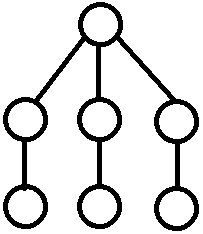
\includegraphics[width=200px,height=200px,keepaspectratio]{vertexdeletionce.png}
			\linespread{0.8}\caption{Counter-example tree}
		\end{figure}
		\begin{figure}[h]
			\centering
			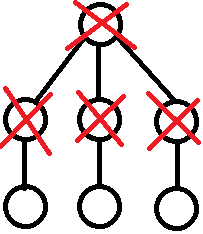
\includegraphics[width=200px,height=200px,keepaspectratio]{vertexdeletioncegreedywrong.png}
			\linespread{0.8}\caption{Greedy algorithm result}
		\end{figure}
		\begin{figure}[h]
			\centering
			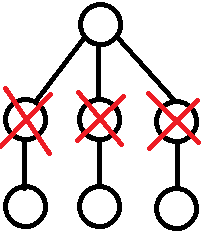
\includegraphics[width=200px,height=200px,keepaspectratio]{vertexdeletionceoptimalright.png}
			\linespread{0.8}\caption{Optimal result}
		\end{figure}
		\clearpage
		The greedy algorithm will start with the vertex at the top as it has the highest degree, and only then delete three vertices that still have $deg(1)$.
		
		But if we look at the optimal way, it is useless and adds an extra vertex to delete, when we could delete the "middle" vertices that have a smaller degree than the top one.
		
	\section{}
		We can represent every point as a vertex, and the distance between two vertices as an edge. So we basically get a complete graph.
		
		We use a matrix representation of the edges, or distance, and sort the rows (or columns).
		
		Then, just go to the middle row (or column), at $n/2$, and give the corresponding vertex.
		
		Since the matrix will be sorted by distances, we know the middle one will include all of the previous half inside its radius distance.
		
		Creating the matrix by traversing the graph and computing the distance is $O(n^2)$.
		Computing the distance is $O(1)$, and you do this for every vertex, for every neighbour, so $O(n(n-1))$. We also do not need to recompute the same edge/distance twice since for every edge it's computed at both vertex but we only need to do it once.
		
	\section{}
		We use the reverse-deletion algorithm to find a spanning tree, except that we force it to keep edges in $F$.
		
		Begin with putting all of the edges in a set.
		Remove one by one the most costly edge left every time but without removing edges in $F$.
		
		We know reverse-deletion gives us the minimum spanning tree.
		In this case, all we are doing is keeping \textit{more} edges (that do not form cycles).
		So either we end up with what the normal algorithm gives, except with extra edges in $F$ (that we are forced to keep), or we delete more edges (the next most costly ones) than what the algorithm would normally give, as to avoid cycles created by edges in $F$ that we wouldn't have in the normal algorithm solution.
		
		Thus, we still get the minimum spanning tree.
	
\end{document}
